\chapter{Analysis of a Horse Movement}
\label{HorseAnalysis}
The movement analysis is a~widely studied problem in many fields. We can measure the movement inside a~laboratory using a~group of (high-speed) cameras or we can use some kind of wearable sensors. The wearable sensors do not require an installation of the cameras so we can achieve higher mobility. A~possible motion tracking solution using wearable sensors is provided by Xsens company \cite{Xsens:MVN}. Other possible solutions are mentioned in chapter \ref{HWavailableSolutions}.

I have selected the movement analysis task for proving the functionality of the \index{SensorBoard}. It means that I will use the \index{SensorBoard} hardware with an existing or a~new algorithm for analyzing the movement. I do not have the other hardware solutions available, so I do not do any measurements for comparison of the results.

The analysis algorithm will be designed to determine the kind of a~movement of a~horse -- stand, walk, trot or gallop.

\section{Definitions of types of the movement}
\label{definitionsOfGaits}
Before we start any analysis, we have to define all the movement types taken into account. First, I will define a~gait in general, and then each type of gait taken into account.

\begin{definition}{\textbf{Gait}}
    \label{def:gait}
    \textit{Gait is the pattern of movement of the limbs of animals, including humans, during locomotion over a~solid substrate. Most animals use a~variety of gaits, selecting gait based on speed, terrain, the need to maneuver, and energetic efficiency.} \cite{Higgins2009}
\end{definition}

I will define each gait as a~sequence of the following symbols. All the definitions I created in this section are based on external sources. \cite{Higgins2009} \cite{Duruttya2005} \cite{Harrisc1993}

\paragraph{List of used symbols in the definitions:}\quad\\
\begin{tabular}{c|p{.9\linewidth}}
    $LF$                   & Left front leg. \\
    $LH$                   & Left hind leg. \\
    $RF$                   & Right front leg. \\
    $RH$                   & Right hind leg. \\
    $\wedge$               & Any leg touched the ground, but we do not know which one. The symbol replaces $\downarrow LF$ or $\downarrow LH$ or $\downarrow RF$ or $\downarrow RH$ symbol. \\
    $\uparrow$             & The leg left the ground and cannot generate acceleration. \\
    $\downarrow$           & The leg touches the ground and generates acceleration (generates a~touch in the signal based on definition \ref{def:touch}). \\
    $\dots$                & The whole movement is repeating forever from this point. \\
    $X, Y$                 & $X$ and $Y$ occurs at the same time or the time difference is lower than $\epsilon$. \\
    $X \cdot Y$            & The time between $X$ and $Y$ is significantly higher than $2\epsilon$, but lower than $\delta$. \\
    $X \sim Y$             & The time between $X$ and $Y$ is significantly higher than $2\delta$, but lower than $\gamma$. \\
    $\gamma$                & It is the longest time when the horse is able to be in the air by his own force. ($\gamma \in \mathbb{R^{+}}$) \\
    $\delta\epsilon$ & $ \exists \delta, \epsilon : 0 \leq \epsilon < 2\epsilon < \delta < 2\delta < \gamma $ \\
\end{tabular}

\subsection{Stand}
\begin{definition}{\textbf{Stand}}
    \label{def:stand}
    A~horse is standing when all its four hoofs are touching the ground. \cite{Harrisc1993}
    
    \begin{enumerate}
        \item The complete definition using the symbols:
        $$ \downarrow RH, \downarrow LH, \downarrow RF, \downarrow LF, \dots $$
        \item With only the detection of touching the ground:
        $$ \downarrow RH, \downarrow LH, \downarrow RF, \downarrow LF, \dots $$
        \item Without knowledge about what leg touched the ground:
        $$ \wedge, \wedge, \wedge, \wedge, \dots $$
        \item Short form:
        $$ \wedge, \dots $$
    \end{enumerate}
\end{definition}

\subsection{Walk}
\begin{definition}{\textbf{Walk}}
    \label{def:walk}
    \textit{The walk is a~four-beat gait that averages about 4 miles per hour (\SI{6.4}{km/h}). When walking, a~horse's legs follow this sequence: left hind leg, left front leg, right hind leg, right front leg, in a~regular 1-2-3-4 beat. At the walk, the horse will alternate between having three or two feet on the ground. A~horse moves its head and neck in a~slight up and down motion that helps maintain balance.} \cite{Harrisc1993}
    
    \begin{enumerate}
        \item The complete definition using the symbols:
        $$ \uparrow RH \sim \downarrow LF \sim \uparrow RF \sim \downarrow RH \sim \uparrow LH \sim \downarrow RF \sim \uparrow LF \sim \downarrow LH \sim \dots $$
        \item With only the detection of touching the ground:
        $$ \downarrow LF \sim \downarrow RH \sim \downarrow RF \sim \downarrow LH \sim \dots $$
        \item Without knowledge about what leg touched the ground:
        $$ \wedge \sim \wedge \sim \wedge \sim \wedge \sim \dots $$
        \item Short form:
        $$ \wedge \sim \dots $$
    \end{enumerate}
\end{definition}

\begin{remark}
    An amble $$\downarrow RH, \downarrow RF, \downarrow LH, \downarrow LF, \dots$$ is not a walk according to the definition \ref{def:walk}, but the parts (3) and (4) count an amble as a walk.
\end{remark}

The figure \ref{fig:walk} shows the horse during walk.

\begin{figure}
	\centering
	\caption{A horse during walk. \cite{Duruttya2005}}
	\label{fig:walk}
	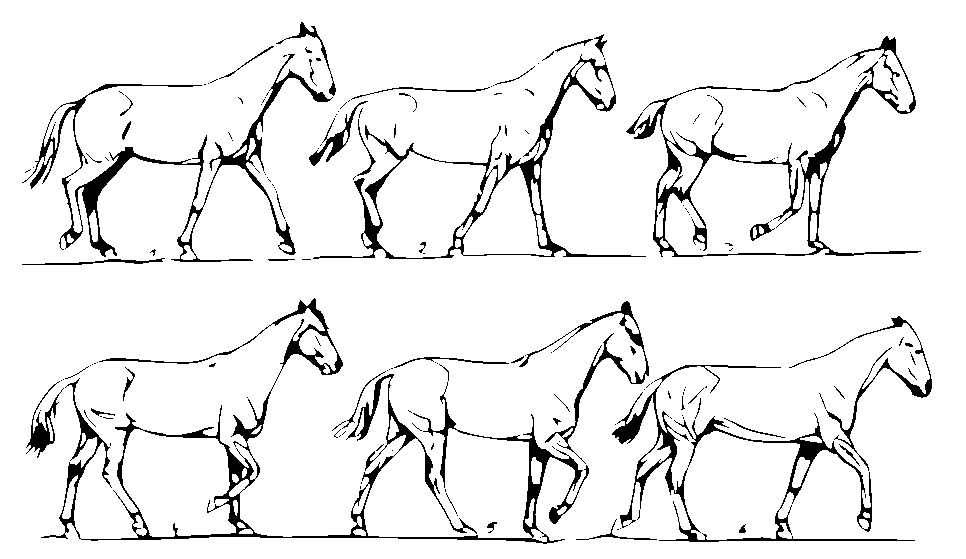
\includegraphics[width=\linewidth]{img/krok.pdf}
\end{figure}

\subsection{Trot}
\begin{definition}{\textbf{Trot}}
    \label{def:trot}
    \textit{The trot is a two-beat gait that has a wide variation in possible speeds, but averages about 8 miles per hour (\SI{13}{km/h}). A very slow trot is sometimes referred to as a jog. An extremely fast trot has no special name, but in harness racing, the trot of a Standardbred is faster than the gallop of the average non-racehorse.} \cite{Harrisc1993}
    
    \begin{enumerate}
        \item The complete definition using the symbols:
        $$ \uparrow RH, \uparrow LF, \downarrow LH, \downarrow RF \sim \downarrow RH, \downarrow LF, \uparrow LH, \uparrow RF \dots $$
        \item With only the detection of touching the ground:
        $$ \downarrow LH, \downarrow RF \sim \downarrow RH, \downarrow LF \dots $$
        \item Without knowledge about what leg touched the ground:
        $$ \wedge, \wedge \sim \wedge, \wedge \sim \dots $$
        \item Short form:
        $$ \wedge, \wedge \sim \dots $$
    \end{enumerate}
\end{definition}

\begin{remark}
    The pace $$\uparrow RH, \uparrow RF, \downarrow LH, \downarrow LF \sim \downarrow RH, \downarrow RF, \uparrow LH, \uparrow LF \dots$$ is not a trot according to this definition, but (3) and (4) count a pace as trot.
\end{remark}

The figure \ref{fig:trot} shows the horse during trot.

\begin{figure}
	\centering
	\caption{A horse during trot. \cite{Duruttya2005}}
	\label{fig:trot}
	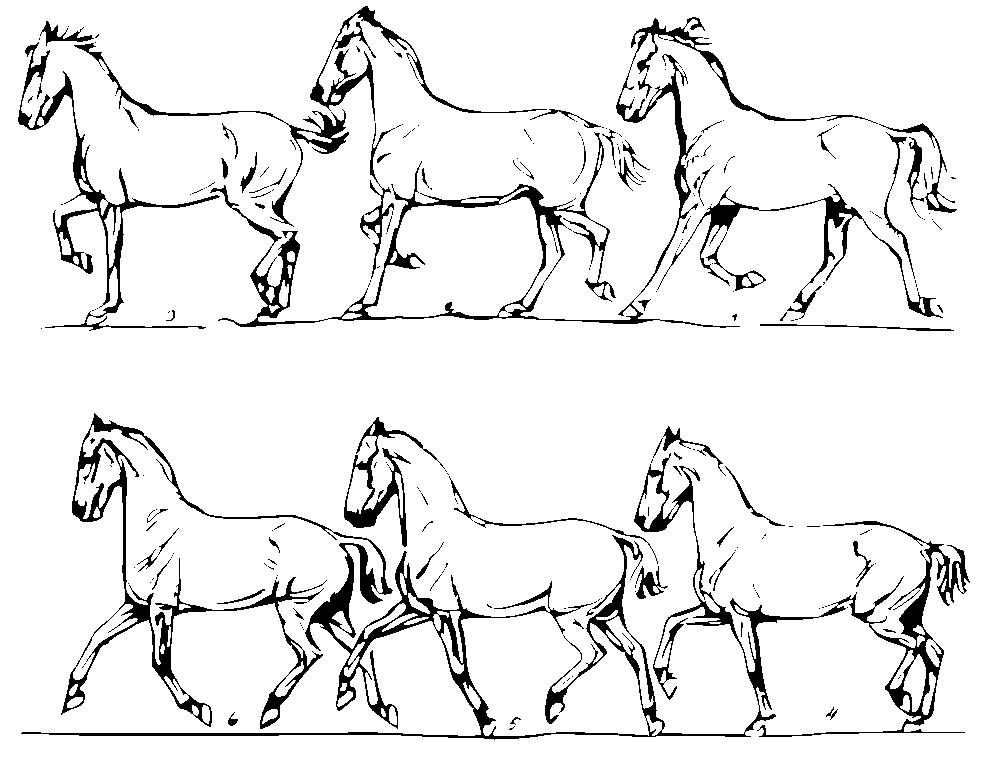
\includegraphics[width=\linewidth]{img/klus.pdf}
\end{figure}

\subsection{Canter}
\begin{definition}{\textbf{Canter}}
    \label{def:canter}
    \textit{The canter is a controlled, three-beat gait that usually is a bit faster than the average trot, but slower than the gallop. The average speed of a canter is \SIrange{16}{27}{km/h} (\SIrange{10}{17}{mph}), depending on the length of the stride of the horse. Listening to a horse canter, one can usually hear the three beats as though a drum had been struck three times in succession. Then there is a rest, and immediately afterward the three-beat occurs again. The faster the horse is moving, the longer the suspension time between the three beats.}
    
    \textit{In the canter, one of the horse's rear legs -- the right rear leg, for example -- propels the horse forward. During this beat, the horse is supported only on that single leg while the remaining three legs are moving forward. On the next beat the horse catches itself on the left rear and right front legs while the other hind leg is still momentarily on the ground. On the third beat, the horse catches itself on the left front leg while the diagonal pair is momentarily still in contact with the ground.} \cite{Harrisc1993}
    
    \begin{enumerate}
        \item Using the symbols (driven by right hand):
        $$ \downarrow RH \cdot \downarrow LH, \downarrow RF \cdot \uparrow RH \cdot \downarrow LF \cdot \uparrow LH \cdot \uparrow RF \cdot \uparrow LF \sim \dots $$
        \item With only the detection of touching the ground (driven by right hand):
        $$ \downarrow RH \cdot \downarrow LH, \downarrow RF \cdot \downarrow LF \sim \dots $$
        \item Without knowledge about what leg touched the ground (driven by right hand):
        $$ \wedge \cdot \wedge, \wedge \cdot \wedge \sim \dots $$
        \item Short form (driven by right hand):
        $$ \wedge \cdot \wedge, \wedge \cdot \wedge \sim \dots $$
        \item Using the symbols (driven by left hand):
        $$ \downarrow LH \cdot \downarrow RH, \downarrow LF \cdot \uparrow LH \cdot \downarrow RF \cdot \uparrow RH \cdot \uparrow LF \cdot \uparrow RF \sim \dots $$
        \item With only the detection of touching the ground (driven by left hand):
        $$ \downarrow LH \cdot \downarrow RH, \downarrow LF \cdot \downarrow RF \sim \dots $$
        \item Without knowledge about what leg touched the ground (driven by left hand):
        $$ \wedge \cdot \wedge, \wedge \cdot \wedge \sim \dots $$
        \item Short form (driven by left hand):
        $$ \wedge \cdot \wedge, \wedge \cdot \wedge \sim \dots $$
    \end{enumerate}
\end{definition}

The figure \ref{fig:canter} shows the horse during canter.

\begin{figure}
	\centering
	\caption{A horse during canter. \cite{Duruttya2005}}
	\label{fig:canter}
	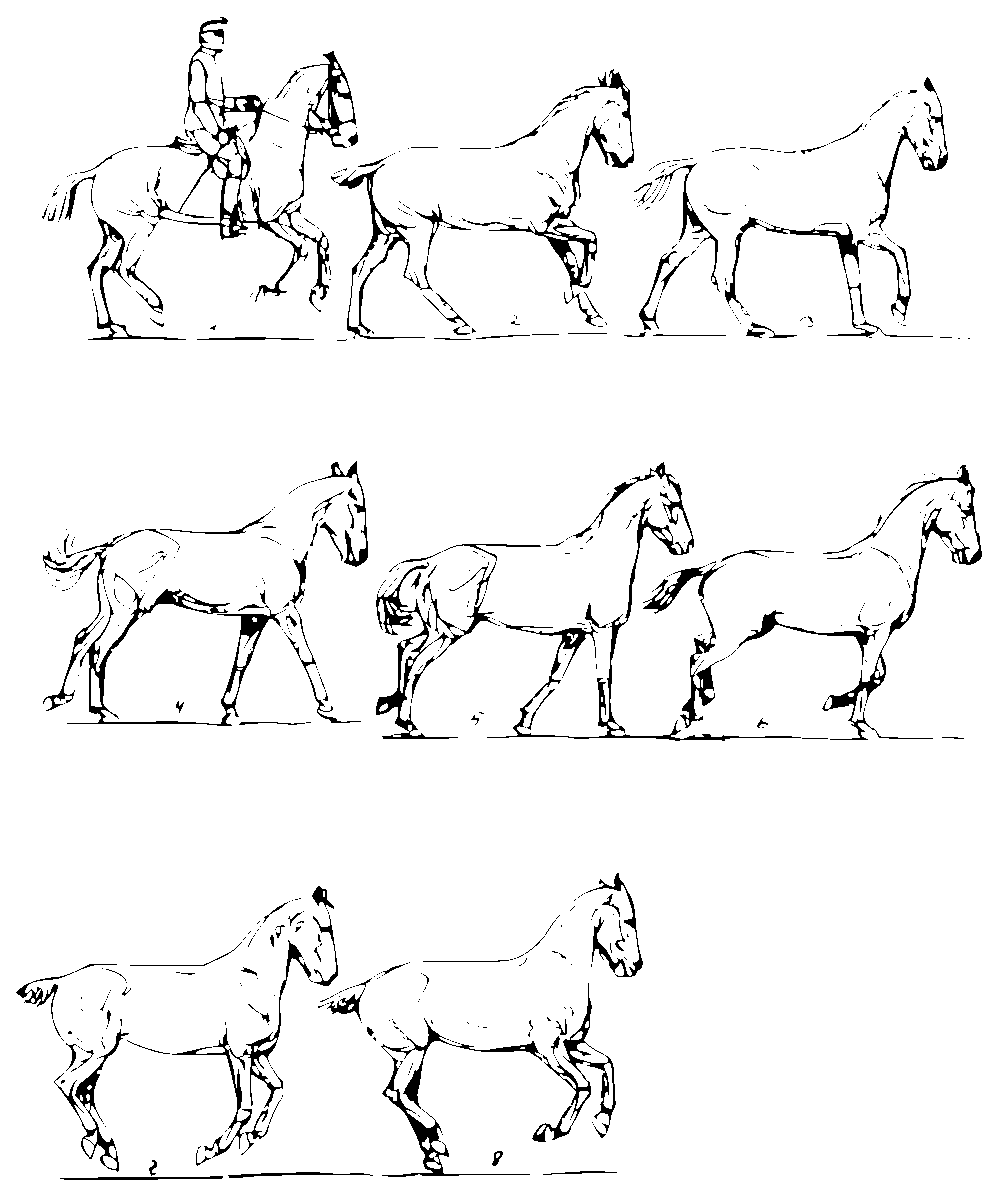
\includegraphics[width=\linewidth]{img/cval.pdf}
\end{figure}

\subsection{Gallop}
\begin{definition}{\textbf{Gallop}}
    \label{def:gallop}
    \textit{The gallop is very much like the canter, except that it is faster, more ground-covering, and the three-beat canter changes to a four-beat gait. It is the fastest gait of the horse, averaging about 25 to 30 miles per hour (\SIrange{40}{48}{km/h}), and in the wild is used when the animal needs to flee from predators or simply cover short distances quickly. Horses seldom will gallop more than 1 or 2 miles (\SI{1.6}{km} or \SI{3.2}{km}) before they need to rest, though horses can sustain a moderately paced gallop for longer distances before they become winded and have to slow down.}
    
    \textit{Like a canter, the horse will strike off with its non-leading hind foot; but the second stage of the canter becomes, in the gallop, the second and third stages because the inside hind foot hits the ground a split second before the outside front foot. Then both gaits end with the striking off of the leading leg, followed by a moment of suspension when all four feet are off the ground. A careful listener or observer can tell an extended canter from a gallop by the presence of the fourth beat.} \cite{Harrisc1993}
    
    \begin{enumerate}
        \item The complete definition using the symbols:
        $$ \downarrow RH \cdot \downarrow LH \cdot \downarrow RF \cdot \uparrow RH \cdot \downarrow LF \cdot \uparrow LH \cdot \uparrow RF \cdot \uparrow LF \sim \dots $$
        \item With only the detection of touching the ground:
        $$ \downarrow RH \cdot \downarrow LH \cdot \downarrow RF \cdot \downarrow LF \sim \dots $$
        \item Without knowledge about what leg touched the ground:
        $$ \wedge \cdot \wedge \cdot \wedge \cdot \wedge \sim \dots $$
        \item Short form:
        $$ \wedge \cdot \wedge \cdot \wedge \cdot \wedge \sim \dots $$
    \end{enumerate}
\end{definition}

\begin{remark}
    The canter and gallop have a very similar definition. We can see that the definitions (2), (3) and (4) are the same for both gaits. So, when we do not measure the complete information, we are not able to distinguish these two types of movement.
\end{remark}

The figure \ref{fig:gallop} shows the horse during gallop.

\begin{figure}
	\centering
	\caption{A horse during gallop. \cite{Duruttya2005}}
	\label{fig:gallop}
	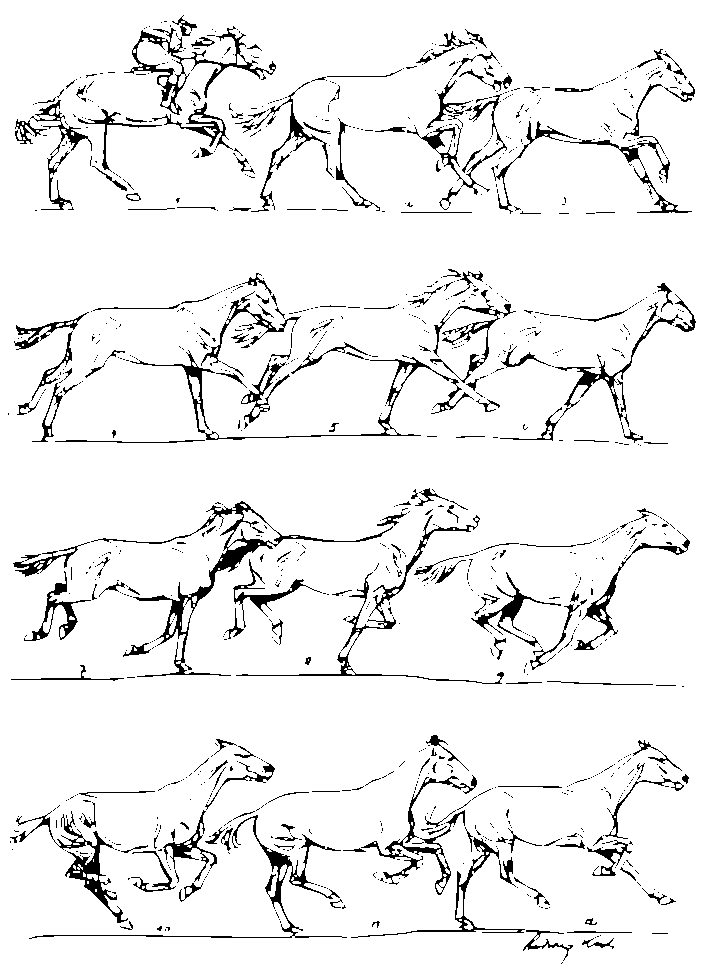
\includegraphics[width=\linewidth]{img/trysk.pdf}
\end{figure}

\section{The input data}
The movement analysis is based on the data from inertial sensors in this task. The input is a stream of values from the triaxial accelerometer, \ac{MEMS} gyroscope and magnetometer at a constant frequency. If we want to run the algorithm on very cheap hardware, we would like to use only values from the accelerometer, gyroscope, or both. The \index{SensorBoard} hardware is able to measure some additional values like relative position to other sensors, sound etc. These values are important, but they are not used in the basic version of the algorithm.

All the data in this chapter were captured during March 2018. The SensorBoard was mounted on the thoroughbread race horse, 14~years old and without movement restrictions. The horse was trained for a recereational riding. The rider has the Basic rider training license obtained from the Czech Riding Federation.

\begin{itemize}
    \item \textbf{Accelerometer:} Values for each axis at frequency \SI{100}{Hz} with maximal range of \SI{\pm 16}{G}.
    \item \textbf{Gyroscope:} Values for each axis at frequency \SI{100}{Hz} with maximal range of $2000 \degree s^{-1}$.
    \item \textbf{Magnetometer:} Values for each axis at frequency \SI{8}{Hz}.
\end{itemize}

\begin{remark}
    When we convert the measured signals to sound, we get interesting results. We have to speed up the signal because we need to move the sound to hearable frequencies. When we listen to the signal, we can hear the differences and later we can learn to distinguish the kind of movement. The figure \ref{accToSound} visualize the conversion process mentioned in this remark.
    
    \begin{figure}[H]
        \centering
        \caption{Conversion of the accelerometer data to hearable sound.}
        \label{accToSound}
        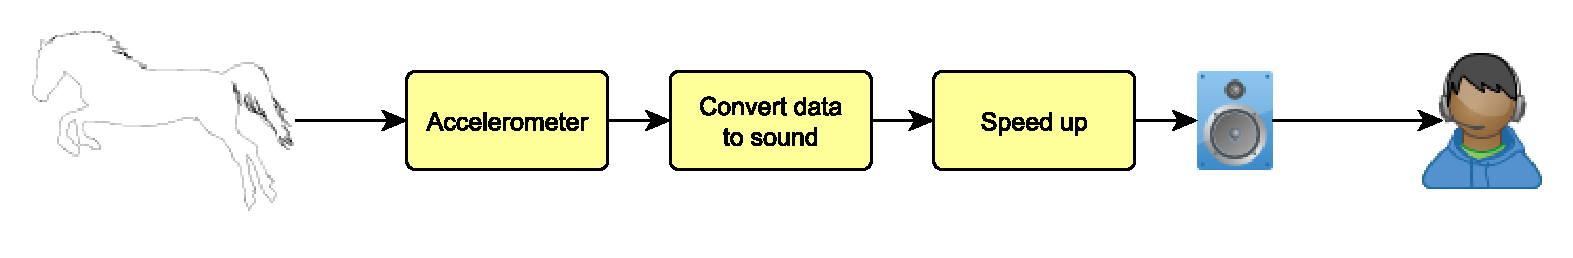
\includegraphics[width=\linewidth]{img/accToSound.pdf}
    \end{figure}
\end{remark}

\subsection{Positions of the sensors}
The position of the sensors on the body is also very important. For example, when the sensor is mounted on the cannon, on the head or on the saddle, the measured data are very different. The figure \ref{fig:differentSensorPosition} shows the differences between the measured data. The visualized values $s$ are computed as sizes of the measured acceleration vectors $\vec{v} = (x,y,z)$:

$$ s = \sqrt{x^{2}+y^{2}+z^{2}} $$

When we have more sensors mounted at different places, we can determine the type of movement more accurately. There is a question if we can determine the type of movement \SI{100}{\%} accurately with using only the inertial sensors. This problem is analyzed later in this chapter.

\begin{figure}
    \centering
    \caption{Different position of the inertial sensors gives different measurements. The~graphs show size of the acceleration vector.}
    \label{fig:differentSensorPosition}
    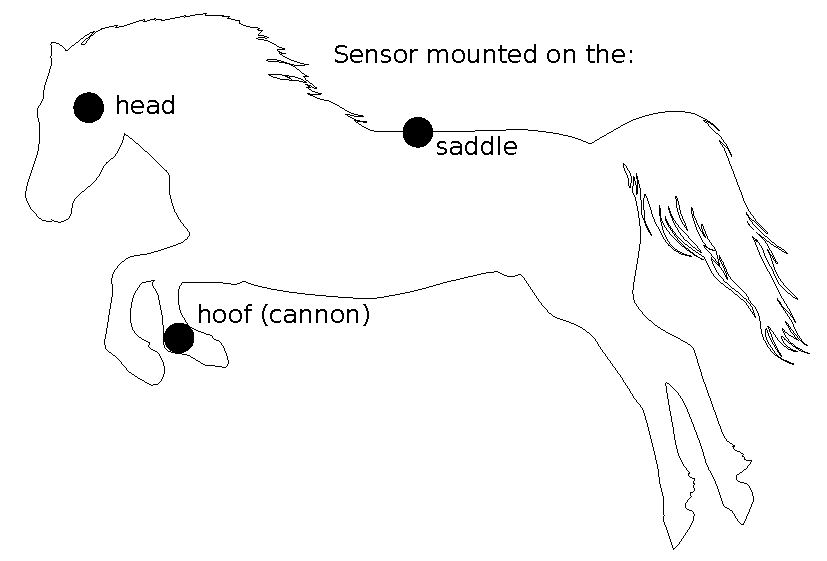
\includegraphics[scale=0.5]{img/sensorMount.pdf} \\
    \includegraphics[width=15cm]{img/walkHead100Hz.eps} \\
    \includegraphics[width=15cm]{img/walkSaddle100Hz.eps} \\
    \includegraphics[width=15cm]{img/walkHoof100Hz.eps}
\end{figure}

\subsection{The measured data as digital signal}
A digital signal is a signal represented by a sequence of discrete values. \cite{DigitalSignalProcessing} The input data fulfill the definition of the digital signal. It means that the algorithm used for the movement analysis is a \ac{DSP} algorithm.

The horse gait is a periodical movement. The period is changing with time, so we cannot specify a constant period for more than one cycle. For example, when the horse is going around, the inner legs do shorter steps than the outer legs. The graph of the measured data in figure \ref{fig:graphPeriodicalMovement} shows the different period of each step.

\begin{figure}
    \centering
    \caption{Detection of the period of the walk. The narrow green line shows the new detected step. The descending green line shows the time when the next step is awaited. The peroid is different in every cycle.}
    \label{fig:graphPeriodicalMovement}
    \includegraphics[width=\linewidth]{img/periodDetection.eps}
\end{figure}

\subsection{Input data requirements}
The digital signals have to be captured in constant frequency. \cite{DSPbook} The frequency must be at least two times higher than the highest frequency in the signal (\ind{Nyquist rate}). \cite{NyquistRate} When the logging frequency is variable, the data gives wrong information about changing the speed of the horse and its steps.

The range of the sensor must be higher than the data range. When this condition is not fulfilled and the algorithm receives saturated values, the output can be negatively affected.

The requirements:
\begin{itemize}
    \item Constant frequency
    \item Not exceeded \ind{Nyquist rate}
    \item No saturated values, all measured data are in a given range
\end{itemize}

\section{Tools for the analysis}
Before choosing the algorithm for the movement determination, we will discuss some options in this section.

\subsection{Step counter}
\label{stepCounter}
A simple step counter is not a good solution for determination of the movement. For example, a slow canter has fewer steps per second than a fast trot. So, the number of steps per second is not an accurate pointer of the type of movement.

The amplitude of each step can help with the movement determination, but it is still not accurate. The canter and trot can have the same amplitudes of their steps.

For an accurate determination, we need to analyze the definition of each kind of movement in detail. The types of gaits are described in section \ref{definitionsOfGaits}. From the definition, the main difference between each gait is in order of hoofs touching the ground. All the other parameters (acceleration in peaks, timing, \dots) can be the same for more than one type of movement. Of course, we probably can find a correlation between the other parameters and the type of movement, but we cannot guarantee the accuracy without any deeper analysis.

When we have a sensor on each cannon with synchronized start and stop, we can distinguish each leg (hoof touching the ground) and get accurate results. When we have only one sensor, for example on the saddle, we still know that any hoof touched the ground, but the sensor measures the values with higher noise and we can capture some false positives. These false positives can negatively affect the final analysis. This method is discussed in detail in section \ref{signalLabelling}. The differences between the measured values on different positions of the sensor are shown in figure \ref{fig:differentSensorPosition}.

\subsection{Spectral analysis}
\label{spectralAnalysis}
The spectral analysis of the measured data can help to find some correlation between the gait type and the frequencies occurred in the digital signal. There is no guarantee that we will find a suitable correlation, but the probability is not low. The visualization of the spectral analysis of the data captured on the saddle is shown in figure \ref{fig:spectralAnalysis}.

\begin{figure}
    \centering
    \caption{Spetral analysis of the variable movement.}
    \label{fig:spectralAnalysis}
    \includegraphics[width=\linewidth]{img/specgramAcc.eps}
\end{figure}

The figure is generated using the \texttt{spectrogram} function in Matlab with \SI{2}{s} Hamming window. The longest step should not be longer than \SI{1}{s}. We can see some sections in the figure that correspond to different gaits.

Now, we can distinguish the sections by some markers. The marker can be, for example, the strongest frequency, average amplitude, occurrence of higher frequencies, etc. Here in this example have marked the highest frequency in figure \ref{fig:spectralHighest}.

\begin{figure}
    \centering
    \caption{Selected strongest frequency from the spectrogram.}
    \label{fig:spectralHighest}
    \includegraphics[width=\linewidth]{img/maxFreq.eps}
\end{figure}

Sometimes, the highest frequency is affected by other factors because the sensor is mounted on the saddle -- far away from the hoofs. I will filter single values that point to the other type of movement than its neighbors. The result is shown in figure \ref{fig:spectralFiltered}.

\begin{figure}
    \centering
    \caption{Strongest frequency from the spectrogram filtered by its neighbors.}
    \label{fig:spectralFiltered}
    \includegraphics[width=\linewidth]{img/filtered.eps}
\end{figure}

Now, we can compare this example analysis to the reality. The figure \ref{fig:spectralMarked} shows the regions marked by colors. Each region with the same color represents the same type of movement.

\begin{figure}
    \centering
    \caption{Strongest frequency from the spectrogram compared to the different types of movement. The types are: blue -- stand; yellow -- walk; green -- trot; violet -- canter}
    \label{fig:spectralMarked}
    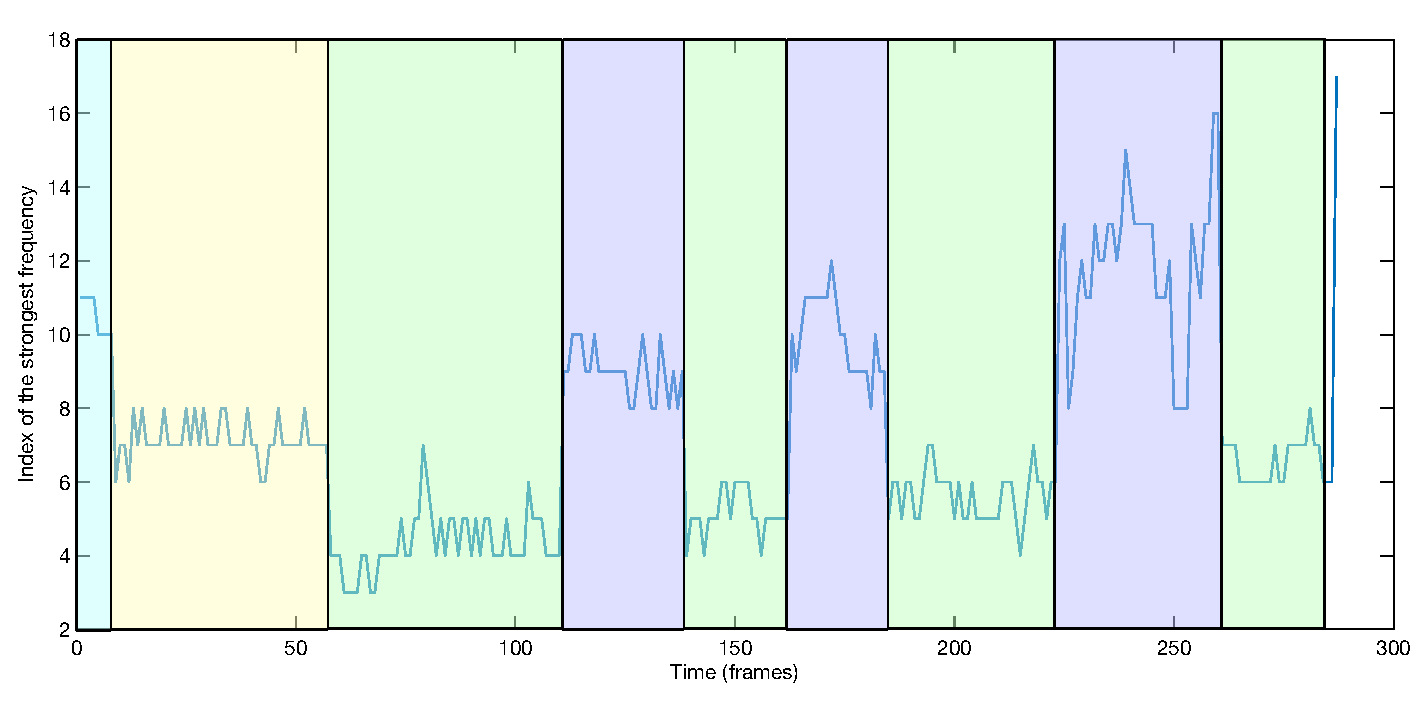
\includegraphics[width=\linewidth]{img/filteredMarked.pdf}
\end{figure}

The analysis gave us suitable results, but we cannot guarantee that the results will be accurate at all times. Different horses will probably need different calibration of the used constants. Of course, we can analyze more factors and then select the most probable movement. We can get almost accurate results with adding more other factors, but we can never guarantee a \SI{100}{\%} correctness of the algorithm. This type of analysis used only the size of the acceleration vector in each time. With other values, we can get more accurate results as well.

I finally did not select this type of analysis because of multiple factors:
\begin{itemize}
    \item The analysis needs higher computation power in comparison to other methods.
    \item The method does not analyze the movement itself, but only its corresponding factors. The method tries to guess the type of the movement based on these factors.
    \item It is hard to add a new type of the movement. The types of gaits are defined inside the algorithm, and there is no possibility to add changes easily.
\end{itemize}

\subsection{Machine learning}
When we have a "hand" created results and their source data we can try to use some machine learning methods. The machine learning methods can be combined with other methods mentioned in this chapter. For example, the spectral analysis from section \ref{spectralAnalysis} can be followed by a neural network, which gives the final results. I was not working with any machine learning algorithm in this thesis and I only mention this type of analysis as a possibility. This analysis again needs a high computation power and there is no guarantee of the accuracy.

\subsection{Looking for structures}
\label{signalLabelling}
The non-trivial digital signal contains some important points, for example, zeros, maximal or minimal values (peaks), inflection points or points that form an obtuse angle with their neighbors in any scale of their plot.

\begin{definition}{\textbf{Peak}}
    A peak $p_t$ of a signal $P = \{p_0, p_1, \dots, p_i, \dots, p_n\}$ is a measured value at time $i$ that fullfills one of these conditions:
    \begin{eqnarray}
    p_{i+1} > p_i \land p_{i-1} > p_i \\
    p_{i+1} < p_i \land p_{i-1} < p_i
    \end{eqnarray}
    
    The peak that fulfills the first condition is called minimal peak and the peak that fulfills the second condition is called maximal peak.
\end{definition}

\begin{definition}{\textbf{Heel}}
    A heel $p_t$ of a signal $P = {p_0, p_1, \dots, p_i, \dots, p_n}$ is a measured value at time $i$ that fullfills one of these conditions:
    \begin{eqnarray}
    (p_{i+1} > p_i \land p_{i-1} = p_i) \land (\exists n : p_n > p_i \land \forall j \in \langle n, i \rangle : p_j = p_i) \\
    (p_{i+1} < p_i \land p_{i-1} = p_i) \land (\exists n : p_n < p_i \land \forall j \in \langle n, i \rangle : p_j = p_i)
    \end{eqnarray}
    
    A heel that fulfills the first condition is a minimal heel and a heel that fulfills the second condition is a maximal heel.
\end{definition}

\begin{definition}{\textbf{Hill}}
    \label{def:hill}
    A hill $H$ is an interval $I_H = \langle i,j \rangle$ in signal $S$ where:
    \begin{enumerate}
        \item The points $s_i$ and $s_j$ are minimal peaks or heels.
        \item $\forall$ peaks $p \in I : p > s_i \land p > s_j$.
    \end{enumerate}
\end{definition}

\begin{remark}
    Size of hill $H$, written $|H|$, is the length of interval $I_H = \langle i,j \rangle$. ($|H| = j - i$)
\end{remark}

\begin{remark}
    A hill $H$ is a part of another hill $G$, written $G \in H$, when the interval $I_G \in I_H$.
\end{remark}

We can look for non-trivial structures like hills, peaks occurred at the same time in different signals or repetition of important points with the same properties. For example, we can count only hills $H$ that are not a part of another hill $F : H \in F$ and do not contain another hill $G$, where $|H| > c \cdot |G|$. The $c \in \mathbb{R}$ is an arbitrary constant that means that the hill $H$ is $c$ times longer than hill $G$.

The figure \ref{fig:peakHeelHill} shows examples of the minimal and maximal peak, heel and hill.

\begin{figure}
    \centering
    \caption{Example of the peak, heel and hill.}
    \label{fig:peakHeelHill}
    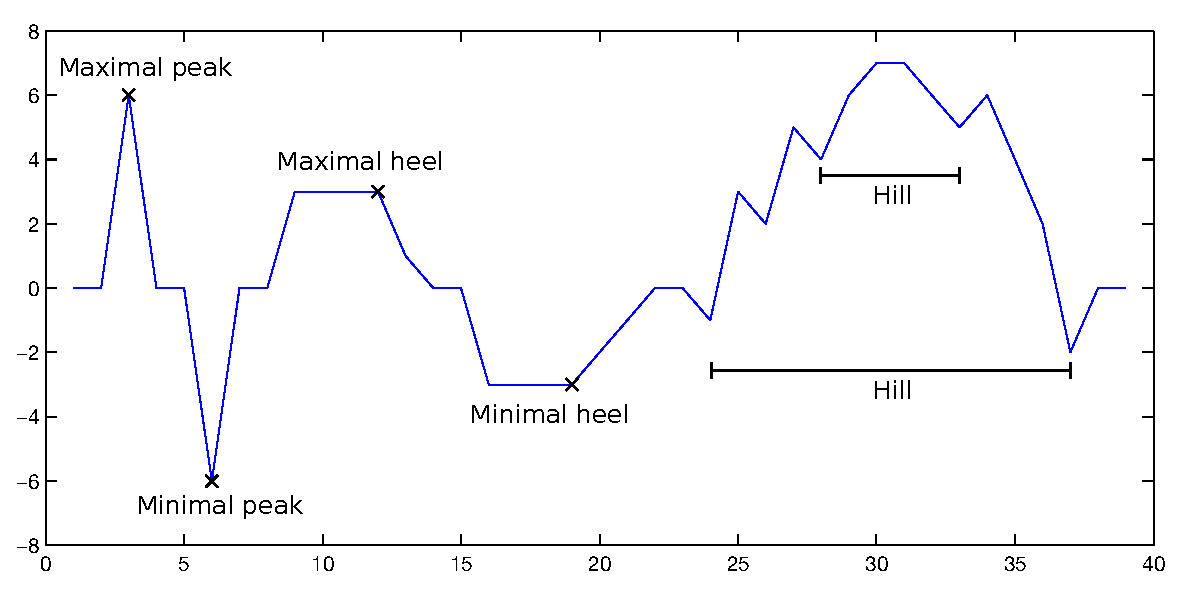
\includegraphics[width=\linewidth]{img/peakHeelHillExample.pdf}
\end{figure}

We can define more structures and use already defined structures in the new definitions. It means that we get a tree of new structures, where the edges are dependencies inside the definitions. The example of this tree is shown in figure \ref{fig:definitionTree}.

\begin{figure}
    \centering
    \caption{Example of the dependencies among definitions displayed as a tree.}
    \label{fig:definitionTree}
    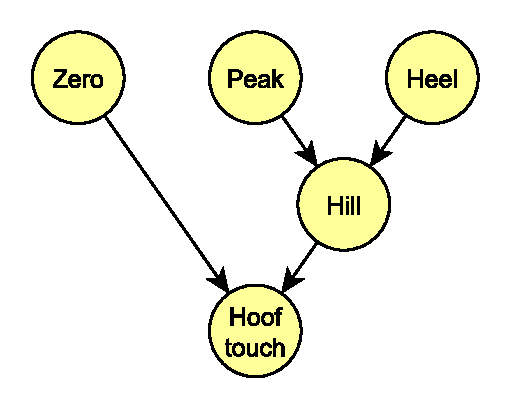
\includegraphics[scale=1]{img/definitionTree.pdf}
\end{figure}

We can combine the definitions with outputs of other types of analysis. The other types can be added as new inputs (sensors). When we add an inaccurate (not \SI{100}{\%} accurate) analysis, we have to take into account that the final result can be inaccurate, too.

The "Looking for structures" analysis is in basics similar to the step counter in section \ref{stepCounter}, but it can be extended to a more powerful tool by the changes mentioned in this section. This is the reason why I finally selected this analysis for implementation into the \index{SensorBoard} hardware. Another reason is based on low \ac{CPU} power requirements and the possibility to get accurate results.

The results are as accurate as the used sensors, definitions and methods. The \SI{100}{\%} accuracy of the algorithm can be achieved by computing the results based on their definitions. Of course, it may be very hard to create an accurate definition of each movement, but when we have a definition, it is easier to test the algorithm against the definition and get indisputable results. The implementation is discussed in section \ref{implementedAnalysis}.

\section{Implemented algorithm}
\label{implementedAnalysis}
I have selected the method described in section \ref{signalLabelling}. The algorithm is implemented as a~\texttt{C++} library, so it can be a part of the firmware of the \index{SensorBoard}, or it can be compiled as a separate application.

\paragraph{Example of the code calling the implemented algorithm:} \quad\\
\Cpp
\begin{lstlisting}
const int frequency = 100; // Hz
HorseAnalysis horse(frequency);

for(;;)
{
	// Load data from sensors to AccX, AccY, AccZ, GyrX, GyrY, GyrZ
	horse.addData(AccX, AccY, AccZ, GyrX, GyrY, GyrZ);
	
	// get elapsed time in milliseconds
	int elapsedTime = horse.elapsedTime();
	// true if horse is moving
	bool isMoving = horse.isMoving();
	// get number of hoof contacts with ground
	int numberOfSteps = horse.numSteps();
	// get type of movement as int representing enum
	int movementType = horse.detectAndNameMovement();
}
\end{lstlisting}

\subsection{Workflow of the algorithm}
The algorithm stores a history of the measured values (5~seconds by default). The history is used for dynamic calibration and as the source for the analysis. The algorithm can run real-time with an approximate latency of one horse's step. So, it cannot detect an unfinished step. The algorithm uses this workflow:
\begin{enumerate}
    \item Read the new input data.
    \item Calibrate the vertical direction and morph the values into the vertical plane.
    \item Mark all the peaks and other interesting points based on their definitions.
    \item Mark more complex structures based on the previously marked points.
    \item Detect a new step. If the new step is detected, continue.\\Otherwise, move to step (1).
    \item Evaluate definitions of the gaits.
    \item Select the most appropriate definition and return the result.
\end{enumerate}

\subsection{Detection of touching the ground}
\begin{definition}{\textbf{Touch}}
    \label{def:touch}
    In this definition, by peak is meant peak or heel. A hill $P$ (based on definition \ref{def:hill}) is a touch, when the hill $P$ does not contain a minimal peak $p_m$ that fulfills:
    \begin{enumerate}
        \item Let $p_i$ and $p_j$ are border peaks of the hill $P$. Let peak $p_x$ is the highest maximal peak~$\in P$. Then:
        $$\exists p_k : p_k > \dfrac{p_x}{2} \land p_m < \dfrac{p_x}{2} \land (i < x < m < k < j \:\lor\: i < k < m < x < j)$$
        \item The hill $P \notin H$, where the hill $H$ is a touch, too.
    \end{enumerate}
\end{definition}

\begin{remark}
    The symbols used in the definition \ref{def:touch} are visualized in figure \ref{fig:touchDefinition}.
\end{remark}

\begin{figure}
    \centering
    \caption{Visualization of the used symbols in definition \ref{def:touch}.}
    \label{fig:touchDefinition}
    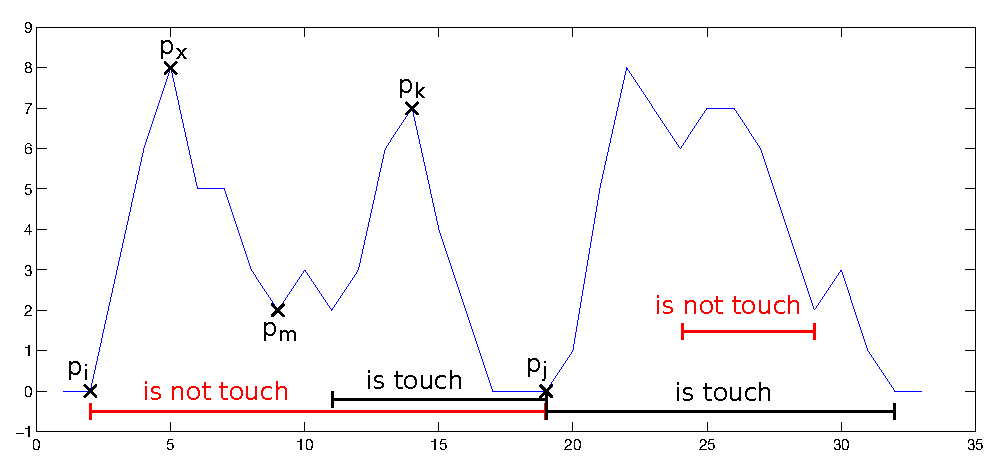
\includegraphics[width=\linewidth]{img/touchHillDefinition.pdf}
\end{figure}

Touching the ground by hoof is detected when the algorithm detects a touch (based on definition \ref{def:touch}).

All the hills $H$ are counted as touching the ground by hoof. We know the
\begin{enumerate}
    \item amplitude -- corresponds to $p_x$,
    \item length -- corresponds to $|H|$,
    \item distance between two hills $H$ and $G$ -- corresponds to $|h_g - h_x|$
\end{enumerate}
The amplitude, length and distance is visualized in figure \ref{fig:touchProperties}.

\begin{figure}
    \centering
    \caption{Visualization of the amplitude, length and distance of the touch (or hill).}
    \label{fig:touchProperties}
    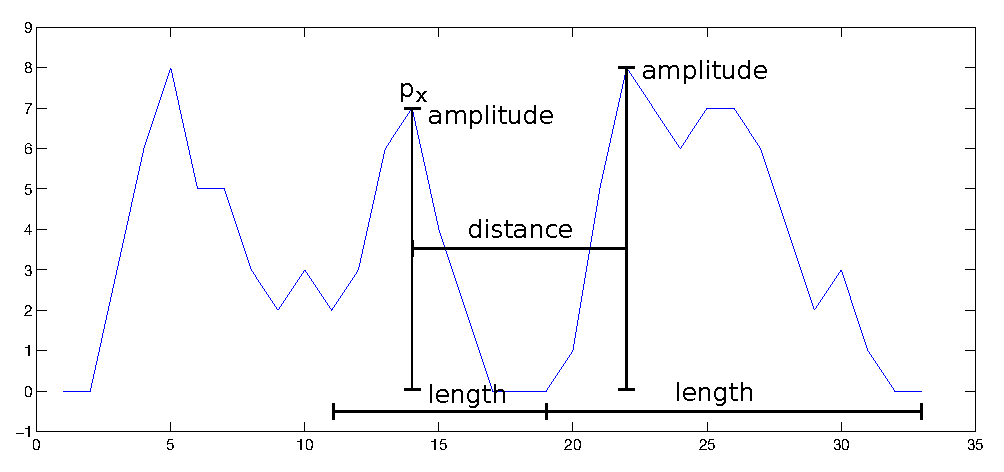
\includegraphics[width=\linewidth]{img/touchHillProperties.pdf}
\end{figure}

\subsection{Definitions of the gaits}
From this point, the algorithm is different when we have the sensor or sensors mounted on the cannon or on the saddle. When the sensor is mounted on the saddle, it can detect touches by all four hoofs, but there may be errors caused by accelerations from different sources. The sensor on the saddle can detect that a hoof touched the ground, but it cannot detect which one.

When we have four sensors -- one on each cannon, the algorithm can detect the movement as accurately as accurate is our definition of the selected movement. The definition defines the step as a structure inside the digital signal, so the definition does not have to exactly correspond to the real steps made by a horse. For example, we can simulate the steps by moving the sensor inside the laboratory without any horse.

Now, I will start with the situation when we have only one sensor. We can use the definitions \ref{def:stand}, \ref{def:walk}, \ref{def:trot}, \ref{def:canter} and \ref{def:gallop}, but only their parts (3) and (4). When the algorithm detects all the touches based on definition \ref{def:touch}, it can measure the amplitudes, lengths of the touches and distances between them. Then the algorithm is able to select the definition, which fits the best to the detected movement. The example of the definitions presented in the source code of the algorithm is shown below.

\paragraph{An example of the definitions used for the analysis:} \quad\\
\Cpp
\begin{lstlisting}
int detectMovement()
{
	if(!isMoving())
		return 0;
	
	// (...)
	
	// First definition
	// -------------------- event ---------------------------
	// if the amplitude of last step is more than 5.0 G,
	// -------------------- action --------------------------
	// increase the probability of gallop (cval = 3)
	if(m_lastStep.amplitude > 5.0 /*G*/)
		prob[3]++;
	
	// Second definition
	// -------------------- event ---------------------------
	// if the time from last step is more than 400 ms,
	// and the amplitude of the last step was less than 2.0 G
	// -------------------- action --------------------------
	// increase the probability of walk (krok = 1)
	if(
		m_time - m_lastStep.time > 400 /*ms*/ &&
		m_lastStep.amplitude < 2.0 /*G*/
	)
		prob[1]++;
	
	// other definitions
	// (...)
	
	return getIndexOfMaxValue(prob, 5 /*size of array prob*/);
}
\end{lstlisting}

When the horse is standing, we cannot detect any touches with significant amplitude. So, all the touches with the amplitude smaller than \SI{1.5}{G} are not counted as touches, and the movement is evaluated as standing.

When we have a sensor on each cannon (or hoof), the algorithm is able to detect which hoof touched the ground. The signal measured on the cannon has much lower noise level than the signal measured on the saddle. When we have multiple sensors, we have to extend the definitions and take into account the part (1) of each definition. Then we get more accurate results with the same algorithm, but we need at least four sensors and the installation time is longer.

\subsection{Possibilities of extension of the algorithm}
The \index{SensorBoard} hardware contains some other useful sensors that can help with the movement analysis. These sensors can be used in  similar way like the accelerometer. Using these sensors is not a part of this thesis.
\begin{itemize}
    \item \textbf{Gyroscope or megnetometer:} can be used as input for sensor fusion and emulation of \ac{AHRS}.
    \item \textbf{DWM1000:} Relative location to other sensors with \SI{300}{m} range and precision \SI{10}{cm}.
    \item \textbf{GPS:} Externally connected GPS with NMEA 2000 output on \SI{3.3}{V} \ac{UART}.
    \item \textbf{Heart rate:} Externally connected heart rate sensor.
\end{itemize}

\subsection{Results}
The results of the analysis is a text file with information about the actual movement type in every second and a \ac{CSV} file with all computed data during the analysis. The example of the text file is shown in figure \ref{fig:textOutputAnalysis}.

\subsection{Comparison of the SensorBoard to MetaWear}
During the work on this thesis, I was measuring the data with two different devices. In the beginning I used the MetaWear \cite{MetaWear} sensor and later the new developed \index{SensorBoard}. Here I will mention some differences I recognized during each measurement process.
\begin{itemize}
    \item The MetaWear sensor was not able to log more than \SI{30}{s} of data at \SI{100}{Hz} frequency. The \index{SensorBoard} logged more than 10 hours and the time depends only on the capacity of the SD card.
    \item The MetaWear sensor was not able to switch off itself. So, the sensor operated only 3 hours after removing from the charger. The \index{SensorBoard} can be switched on or off manually and it operates about 10 hours until the battery is discharged.
    \item The MetaWear sensor has a Bluetooth connection that can transmit approximately at \SI{2}{m} range. The \index{SensorBoard} transmits approximately in \SI{25}{m} range.
    \item The MetaWear sensor is smaller than \index{SensorBoard}. The dimensions of the MetaWear are approximately twice smaller than the SesnroBoard prototype.
\end{itemize}

\begin{figure}[H]
	\centering
	\caption{Example of the text output of the selected movement analysis.}
	\label{fig:textOutputAnalysis}
	\begin{verbatim}
	(...)
	Second   55: moving yes, steps   93, klus , ...
	Second   56: moving yes, steps   95, klus , ...
	Second   57: moving yes, steps   97, klus , ...
	Second   58: moving yes, steps   99, krok , ...
	Second   59: moving yes, steps  101, krok , ...
	Second   60: moving yes, steps  102, krok , ...
	Second   61: moving no , steps  103, krok , ...
	Second   62: moving no , steps  103, stani, ...
	Second   63: moving yes, steps  103, stani, ...
	Second   64: moving no , steps  104, stani, ...
	(...)
	\end{verbatim}
	\raggedright
	\quad\\The names of the movement are in Czech language for easier testing in the Czech environment. The translation is:\\"stani"~--~stand; "krok"~--~walk; "klus"~--~trot, "cval"~--~canter.
\end{figure}

The \ac{CSV} output can be visualized into a graph for easier orientation in the values. The columns represent selected variables inside the analysis. An example of this graph is shown in figure \ref{fig:graphSelectedAnalysis}.

\begin{figure}[H]
	\centering
	\caption{An example of the graph generated from the CSV file given as output of the analysis.}
	\label{fig:graphSelectedAnalysis}
	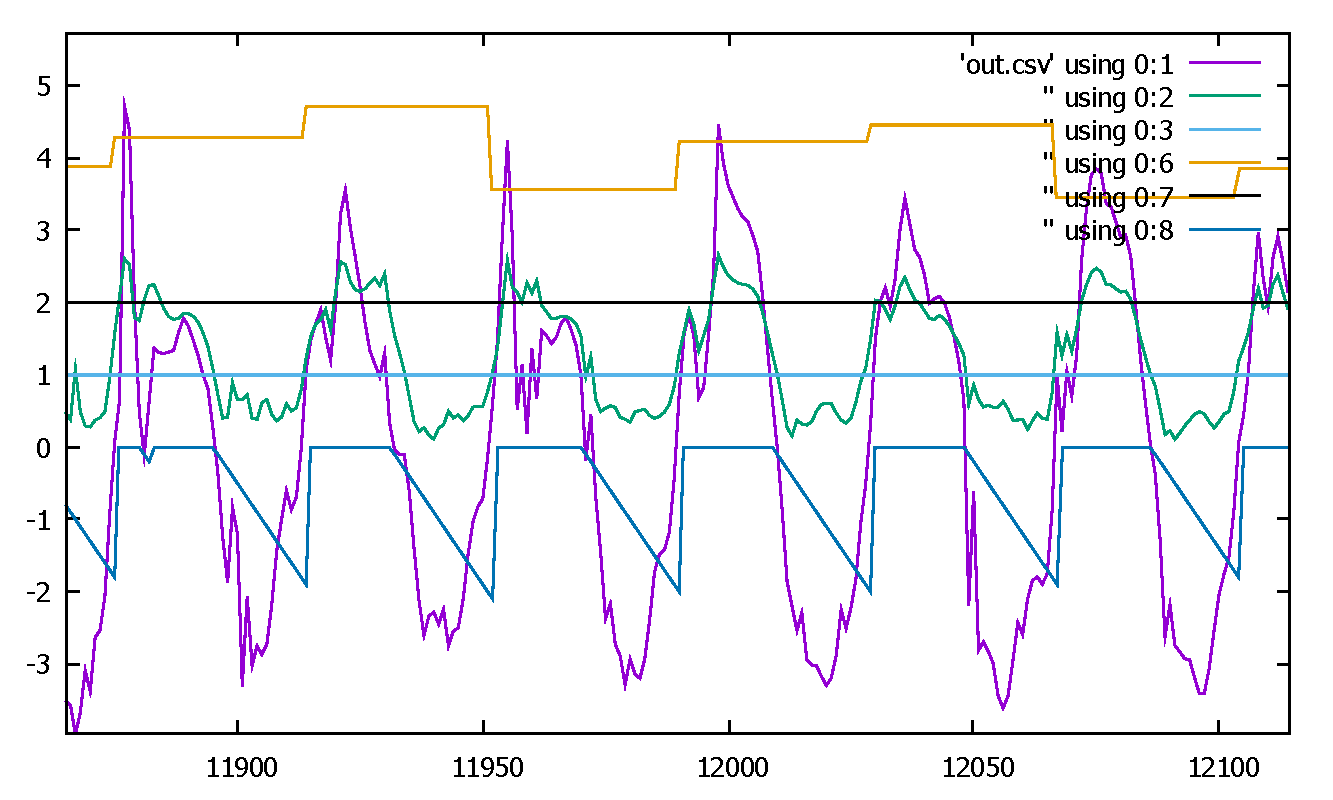
\includegraphics[width=\linewidth]{img/outputHorseAnalysisZoom.pdf}
\end{figure}
